\documentclass{beamer}

\usepackage[slovene]{babel}
\usepackage{amsfonts,amssymb}
\usepackage[utf8]{inputenc}
\usepackage{lmodern}
\usepackage[T1]{fontenc}

\usefonttheme[onlymath]{serif}

\usetheme{Warsaw}

\def\N{\mathbb{N}} % mnozica naravnih stevil
\def\Z{\mathbb{Z}} % mnozica celih stevil
\def\Q{\mathbb{Q}} % mnozica racionalnih stevil
\def\R{\mathbb{R}} % mnozica realnih stevil
\def\C{\mathbb{C}} % mnozica kompleksnih stevil


\def\qed{$\hfill\Box$}   % konec dokaza
\newtheorem{izrek}{Izrek}
\newtheorem{trditev}{Trditev}
\newtheorem{posledica}{Posledica}
\newtheorem{lema}{Lema}
\newtheorem{definicija}{Definicija}
\newtheorem{opomba}{Opomba}
\newtheorem{primer}{Primer}
\newtheorem{zgled}{Zgled}
\newtheorem{zgledi}{Zgledi uporabe}
\newtheorem{zglediaf}{Zgledi aritmetičnih funkcij}
\newtheorem{oznaka}{Oznaka}

\title{Metrična dimenzija grafa deliteljev niča}
\author{Tadeja Možina}

\institute{Mentor: izr.~prof.~dr.~David Dolžan\\
Fakulteta za matematiko in fiziko}
\date{4.\ december 2023}

\begin{document}


%%%%%%%%%%%%%%%%%%%%%%%%%%%%%%%%%%%%%%%%%%%%%%%%%%%%%%%%%%%%%%%%%%%%%

\begin{frame}
\titlepage
\end{frame}

%%%%%%%%%%%%%%%%%%%%%%%%%%%%%%%%%%%%%%%%%%%%%%%%%%%%%%%%%%%%%%%%%%%%%


%%%%%%%%%%%%%%%%%%%%%%%%%%%%%%%%%%%%%%%%%%%%%%%%%%%%%%%%%%%%%%%%%%%%%

\begin{frame}
    \begin{definicija}
        Naj bo R kolobar in $Z(R)$ njegova množica deliteljev niča.
        \emph{Graf deliteljev niča kolobarja R} je enostaven neusmerjen graf z množico
        vozlišč $Z^{*}(R) = Z(R)\setminus\{0\} $, kjer sta dve različni vozlišči $a,b \in Z^{*}(R) $
        povezani natanko tedaj, ko je $ab = 0$ ali $ba = 0$. Označimo ga z $\Gamma(R)$.
    \end{definicija}
    
\end{frame}
    
%%%%%%%%%%%%%%%%%%%%%%%%%%%%%%%%%%%%%%%%%%%%%%%%%%%%%%%%%%%%%%%%%%%%%

\begin{frame}
    
    \begin{zgled}
        Graf deliteljev niča $\Z_{10}$. Množica njegovih vozlišč je 
        $V(\Gamma(\Z_{10})) = Z^{*}(\Z_{10}) = \{2, 4, 5, 6, 8\}$, množica povezav pa 
        je enaka $E(\Gamma(\Z_{10})) = \{2 \sim 5, 4 \sim 5, 6 \sim 5, 8 \sim 5\}$
    \end{zgled}
    \begin{center}
        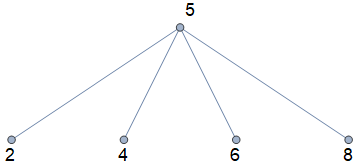
\includegraphics[width=5cm, height=5cm]{z10.png}
    \end{center}
    \begin{center}
        $\Gamma(\Z_{10})$
    \end{center}
    
\end{frame}
    
%%%%%%%%%%%%%%%%%%%%%%%%%%%%%%%%%%%%%%%%%%%%%%%%%%%%%%%%%%%%%%%%%%%%%
    
\begin{frame}
    
    \begin{definicija}
        Naj bo $W = \{ w_1,w_2, \ldots, w_k \}$ urejena podmnožica množice $V(\Gamma)$ in 
        $v \in V(\Gamma)$. Potem 
        se $k$-dimenzionalni vektor \\
        $r(v|W)=( d(v,w_1), \ldots, d(v,w_k) )$ imenuje 
        predstavitev $v$ glede na množico $W$. 
      
    \end{definicija}
    
\end{frame}
    
%%%%%%%%%%%%%%%%%%%%%%%%%%%%%%%%%%%%%%%%%%%%%%%%%%%%%%%%%%%%%%%%%%%%%

\begin{frame}
    
    \begin{zgled}
        Graf deliteljev niča $\Z_{10}$ in množica $W = \{2,4,5\}$.\\
        Predstavitve glede na $W$:\\
        $r(2|W)=( d(2,2), d(2,4), d(2,5) ) = ( 0, 2, 1 )$,
        $r(4|W)=( d(4,2), d(4,4), d(4,5) ) = ( 2, 0, 1 )$,
        $r(5|W)=( d(5,2), d(5,4), d(5,5) ) = ( 1, 1, 0 )$,
        $r(6|W)=( d(6,2), d(6,4), d(6,5) ) = ( 2, 2, 1 )$ in 
        $r(8|W)=( d(8,2), d(8,4), d(8,5) ) = ( 2, 2, 1 )$.
    \end{zgled}
    \begin{center}
        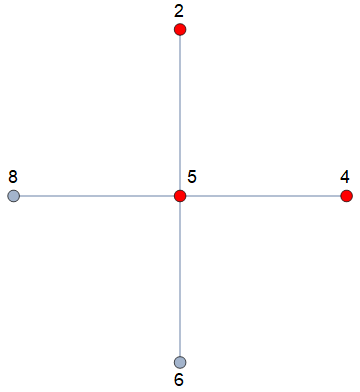
\includegraphics[width=4cm, height=4cm]{z10W1.png}
    \end{center}
    
\end{frame}
    
%%%%%%%%%%%%%%%%%%%%%%%%%%%%%%%%%%%%%%%%%%%%%%%%%%%%%%%%%%%%%%%%%%%%%

\begin{frame}
    
    \begin{definicija}
        Množici $W$ pravimo \emph{rešljiva množica grafa $\Gamma$}, če imata poljubni različni 
        vozlišči v $V(\Gamma)$ različni predstavitvi glede na $W$. Če je $W$ rešljiva množica 
        z najmanjšo močjo, ji pravimo \emph{baza $\Gamma$}.
    \end{definicija}

    \begin{definicija}
        \emph{Metrična dimenzija grafa $\Gamma$} je moč njegove baze. Označimo jo z $dim(\Gamma)$.
    \end{definicija}
    
\end{frame}

%%%%%%%%%%%%%%%%%%%%%%%%%%%%%%%%%%%%%%%%%%%%%%%%%%%%%%%%%%%%%%%%%%%%%

\begin{frame}
    
    \begin{zgled}
        Graf deliteljev niča $\Z_{10}$ in množica $W_2 = \{2,4,6\}$.\\
        Predstavitve glede na $W_2$:\\
        $r(2|W_2)=( d(2,2), d(2,4), d(2,6) ) = ( 0, 2, 2 )$,
        $r(4|W_2)=( d(4,2), d(4,4), d(4,6) ) = ( 2, 0, 2 )$,
        $r(5|W_2)=( d(5,2), d(5,4), d(5,6) ) = ( 1, 1, 1 )$,
        $r(6|W_2)=( d(6,2), d(6,4), d(6,6) ) = ( 2, 2, 0 )$ in 
        $r(8|W_2)=( d(8,2), d(8,4), d(8,6) ) = ( 2, 2, 2 )$.
    \end{zgled}
    \begin{center}
        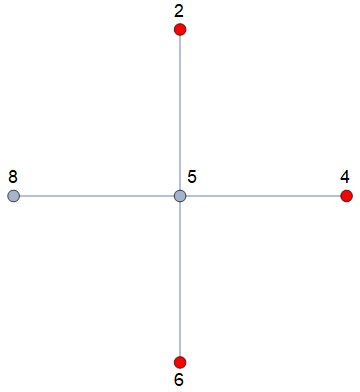
\includegraphics[width=4cm, height=4cm]{z10W2.png}
    \end{center}
    
\end{frame}

%%%%%%%%%%%%%%%%%%%%%%%%%%%%%%%%%%%%%%%%%%%%%%%%%%%%%%%%%%%%%%%%%%%%%

%%%%%%%%%%%%%%%%%%%%%%%%%%%%%%%%%%%%%%%%%%%%%%%%%%%%%%%%%%%%%%%%%%%%%

\begin{frame}
    \frametitle{Kolobarji ostankov}
    \begin{trditev}
        Naj bo $n$ produkt dveh različnih praštevil, $n = p_1 \cdot p_2$. Potem je 
        $dim(\Gamma(\Z_{n})) = p_1 + p_2 - 4$.
    \end{trditev}
    
\end{frame}
    
%%%%%%%%%%%%%%%%%%%%%%%%%%%%%%%%%%%%%%%%%%%%%%%%%%%%%%%%%%%%%%%%%%%%%

\begin{frame}
    \frametitle{Kolobarji ostankov}
    \begin{zgled}
        Praštevilski razcep $10$ je $10 = 2\cdot5$, torej je 
        $dim(\Gamma(\Z_{10})) = 2 + 5 - 4 = 3$.
    \end{zgled}
    \begin{center}
        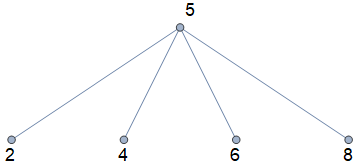
\includegraphics[width=5cm, height=5cm]{z10.png}
    \end{center}
    
\end{frame}    

%%%%%%%%%%%%%%%%%%%%%%%%%%%%%%%%%%%%%%%%%%%%%%%%%%%%%%%%%%%%%%%%%%%%%

\begin{frame}
    \frametitle{Kolobarji ostankov}
    \begin{trditev}
        Naj bo $p$ praštevilo.
    \begin{enumerate}
        \item Če je $n = p^2$ in $p > 2$, potem je $dim(\Gamma(\Z_{n})) = p - 2$,
        \item Če je $n = p^k$ in $k \geq 3$, potem je $dim(\Gamma(\Z_{n})) = p^{k-1} - k$.
    \end{enumerate}
    \end{trditev}
    
\end{frame}

%%%%%%%%%%%%%%%%%%%%%%%%%%%%%%%%%%%%%%%%%%%%%%%%%%%%%%%%%%%%%%%%%%%%%

\begin{frame}
    \frametitle{Kolobarji ostankov}
    \begin{izrek}
        Naj bo $n = \prod_{i = 1}^{r}p_i^{n_i}$ praštevilski razcep $n$. Če je $r \geq 2$ in 
        $\sum_{i=1}^{r}n_i \geq 3$, potem je 
        \begin{equation*}
            dim(\Gamma(\Z_{n})) = n - \varphi(n) - \prod_{i = 1}^{r}(n_i + 1) + 1,
        \end{equation*}
        kjer je $\varphi(n)$ Eulerjeva funkcija $\varphi$.
    \end{izrek}
    
\end{frame}

%%%%%%%%%%%%%%%%%%%%%%%%%%%%%%%%%%%%%%%%%%%%%%%%%%%%%%%%%%%%%%%%%%%%%

\begin{frame}
    \frametitle{Kolobarji ostankov}
    \begin{zgled}
        Graf deliteljev niča $\Z_{12}$. Praštevilski razcep $12$ je $12 = 2^2 \cdot 3^1$, torej je \\
        $dim(\Gamma(\Z_{12})) = 12 - \varphi(12) - (2 + 1)\cdot(1 + 1) + 1 = 12 - 4 - 6 + 1 = 3$.
    \end{zgled}
    \begin{center}
        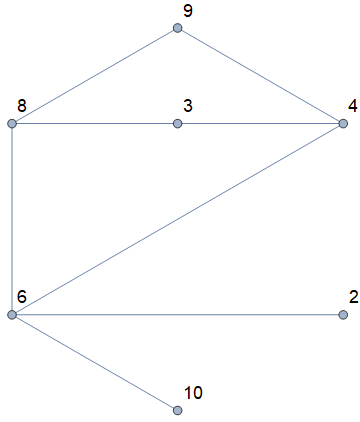
\includegraphics[width=3.5cm, height=4.8cm]{z12.png}
    \end{center}
    \begin{center}
        $\Gamma(\Z_{12})$
    \end{center}
    
\end{frame}    

%%%%%%%%%%%%%%%%%%%%%%%%%%%%%%%%%%%%%%%%%%%%%%%%%%%%%%%%%%%%%%%%%%%%%

%%%%%%%%%%%%%%%%%%%%%%%%%%%%%%%%%%%%%%%%%%%%%%%%%%%%%%%%%%%%%%%%%%%%%

\begin{frame}
    \frametitle{Kolobarji matrik}
    Naj bo $K$ končno polje, $|K| = k$. Označimo:
    \begin{itemize}
        \item kolobar $n \times n$ matrik nad $K$ z $M_n(K)$
        \item $n \times n$ matrike ranga $r$ nad $K$ z $Mat_n^r(K)$
        \item moč $Mat_n^r(K)$ z $m_k(n,r)$
    \end{itemize}

    \begin{izrek}
        Naj bo $|K| = k \geq 3$. Potem je \\
        $dim(\Gamma(M_n(K))) = k^{n^2} - \sum_{i=1}^{n}\frac{m_k(n,i)}{m_k(i,i)} - m_k(n,n)$.
    \end{izrek}

    \begin{izrek}
        Naj bo $n \geq 3$ in $|K| = k = 2$. Potem je \\
        $dim(\Gamma(M_n(K))) = 2^{n^2} - \sum_{i=1}^{n}\frac{m_2(n,i)}{m_2(i,i)} - m_2(n,n)$.
    \end{izrek}
    
\end{frame}  
    
%%%%%%%%%%%%%%%%%%%%%%%%%%%%%%%%%%%%%%%%%%%%%%%%%%%%%%%%%%%%%%%%%%%%%

\begin{frame}
    \frametitle{Kolobarji matrik}
    \begin{trditev}
        $dim(\Gamma(M_2(\Z_2))) = 3$.
    \end{trditev}

    \begin{zgled}
        $\Gamma(M_2(\Z_2))$.
    \end{zgled}
    \begin{center}
        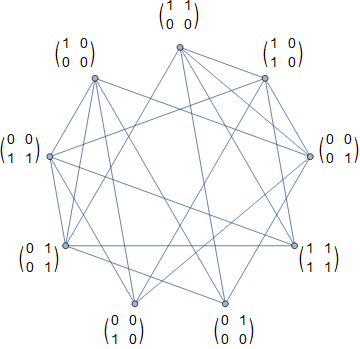
\includegraphics[width=5cm, height=5cm]{m2(2).png}
    \end{center}
    
\end{frame} 

%%%%%%%%%%%%%%%%%%%%%%%%%%%%%%%%%%%%%%%%%%%%%%%%%%%%%%%%%%%%%%%%%%%%%
\end{document}